%Version 3 October 2023
% See section 11 of the User Manual for version history
%
%%%%%%%%%%%%%%%%%%%%%%%%%%%%%%%%%%%%%%%%%%%%%%%%%%%%%%%%%%%%%%%%%%%%%%
%%                                                                 %%
%% Please do not use \input{...} to include other tex files.       %%
%% Submit your LaTeX manuscript as one .tex document.              %%
%%                                                                 %%
%% All additional figures and files should be attached             %%
%% separately and not embedded in the \TeX\ document itself.       %%
%%                                                                 %%
%%%%%%%%%%%%%%%%%%%%%%%%%%%%%%%%%%%%%%%%%%%%%%%%%%%%%%%%%%%%%%%%%%%%%

%%\documentclass[referee,sn-basic]{sn-jnl}% referee option is meant for double line spacing

%%=======================================================%%
%% to print line numbers in the margin use lineno option %%
%%=======================================================%%

%%\documentclass[lineno,sn-basic]{sn-jnl}% Basic Springer Nature Reference Style/Chemistry Reference Style

%%======================================================%%
%% to compile with pdflatex/xelatex use pdflatex option %%
%%======================================================%%

%%\documentclass[pdflatex,sn-basic]{sn-jnl}% Basic Springer Nature Reference Style/Chemistry Reference Style


%%Note: the following reference styles support Namedate and Numbered referencing. By default the style follows the most common style. To switch between the options you can add or remove �Numbered� in the optional parenthesis. 
%%The option is available for: sn-basic.bst, sn-vancouver.bst, sn-chicago.bst%  
 
%%\documentclass[sn-nature]{sn-jnl}% Style for submissions to Nature Portfolio journals
%%\documentclass[sn-basic]{sn-jnl}% Basic Springer Nature Reference Style/Chemistry Reference Style
\documentclass[sn-mathphys-num]{sn-jnl}% Math and Physical Sciences Numbered Reference Style 
%%\documentclass[sn-mathphys-ay]{sn-jnl}% Math and Physical Sciences Author Year Reference Style
%%\documentclass[sn-aps]{sn-jnl}% American Physical Society (APS) Reference Style
%%\documentclass[sn-vancouver,Numbered]{sn-jnl}% Vancouver Reference Style
%%\documentclass[sn-apa]{sn-jnl}% APA Reference Style 
%%\documentclass[sn-chicago]{sn-jnl}% Chicago-based Humanities Reference Style

%%%% Standard Packages
%%<additional latex packages if required can be included here>

\usepackage{graphicx}%
\usepackage{multirow}%
\usepackage{amsmath,amssymb,amsfonts}%
\usepackage{amsthm}%
\usepackage{mathrsfs}%
\usepackage[title]{appendix}%
\usepackage{xcolor}%
\usepackage{textcomp}%
\usepackage{manyfoot}%
\usepackage{booktabs}%
\usepackage{algorithm}%
\usepackage{algorithmicx}%
\usepackage{algpseudocode}%
\usepackage{listings}%
%%%%

%%%%%=============================================================================%%%%
%%%%  Remarks: This template is provided to aid authors with the preparation
%%%%  of original research articles intended for submission to journals published 
%%%%  by Springer Nature. The guidance has been prepared in partnership with 
%%%%  production teams to conform to Springer Nature technical requirements. 
%%%%  Editorial and presentation requirements differ among journal portfolios and 
%%%%  research disciplines. You may find sections in this template are irrelevant 
%%%%  to your work and are empowered to omit any such section if allowed by the 
%%%%  journal you intend to submit to. The submission guidelines and policies 
%%%%  of the journal take precedence. A detailed User Manual is available in the 
%%%%  template package for technical guidance.
%%%%%=============================================================================%%%%

%% as per the requirement new theorem styles can be included as shown below
\theoremstyle{thmstyleone}%
\newtheorem{theorem}{Theorem}%  meant for continuous numbers
%%\newtheorem{theorem}{Theorem}[section]% meant for sectionwise numbers
%% optional argument [theorem] produces theorem numbering sequence instead of independent numbers for Proposition
\newtheorem{proposition}[theorem]{Proposition}% 
%%\newtheorem{proposition}{Proposition}% to get separate numbers for theorem and proposition etc.

\theoremstyle{thmstyletwo}%
\newtheorem{example}{Example}%
\newtheorem{remark}{Remark}%

\theoremstyle{thmstylethree}%
\newtheorem{definition}{Definition}%

\raggedbottom
%%\unnumbered% uncomment this for unnumbered level heads

\begin{document}

\title[Towards Transparency and Knowledge Exchange in AI-assisted Data Analysis Code Generation]{Towards Transparency and Knowledge Exchange in AI-assisted Data Analysis Code Generation}

%%=============================================================%%
%% GivenName	-> \fnm{Joergen W.}
%% Particle	-> \spfx{van der} -> surname prefix
%% FamilyName	-> \sur{Ploeg}
%% Suffix	-> \sfx{IV}
%% \author*[1,2]{\fnm{Joergen W.} \spfx{van der} \sur{Ploeg} 
%%  \sfx{IV}}\email{iauthor@gmail.com}
%%=============================================================%%

\author[1,2]{Robert Haase}
\email{robert.haase@uni-leipzig.de}

\affil[1]{Data Science Center, Leipzig University, Humboldtstra{\ss}e 25, 04105 Leipzig, Germany}
\affil[2]{Center for Scalable Data Analytics and Artificial Intelligence (ScaDS.AI) Dresden / Leipzig}

%%==================================%%
%% Sample for unstructured abstract %%
%%==================================%%

\abstract{

Todo: Enter standfirst here.

}

\maketitle

Generative artificial intelligence (AI) and Large Language Models (LLMs) in particular are changing the way we do data science. Most prominently, scientists use the technology for interacting with scientific data \cite{Royer2023}, answer data analysis questions \cite{Lai2022DS1000, lei2024bioimage}, generate data analysis code \cite{Royer2024, benchmark_llm_bia, chen2021evaluating}, and [re-]write scientific manuscripts \cite{lu2024aiscientist}. Unfortunately, the prompts sent to LLMs are commonly not conserved, and thus, at the time of publication, it might be hard to differentiate human-made and AI-generated parts of the scientific work. A professional peer-review system, for documenting how LLM-generated code was prompted for, and which human reviewed it, is not established in contemporary scientific culture. However, such systems do exist for collaborative code editing involving multiple humans. For example, the source code repositories GitHub and GitLab are well-established in the open-source software community for discussing issues and potential solutions, building code together, and for peer-reviewing contents. As it was shown before that LLMs can solve real-world GitHub issues \cite{jimenez2024swebenchlanguagemodelsresolve}, developing an AI-assistant that interacts with humans directly within the GitHub platform is the obvious next step. 

Here, I present git-bob, an implementation of an LLM-based AI-assistant that can respond to GitHub issues, discuss potential solutions with humans iteratively, write code for them, and submit it as pull-request to be reviewed by humans. It is technically similar to various online services for data analysis such as the OpenAI ChatGPT Data Analyst or GitHub Copilot Workflows, with three major differences. First, multiple humans can interact with git-bob in one communication thread. This allows bringing together domain specialists, such as life scientists, data-analysts and the AI-assistant in one discussion, stimulating knowledge exchange on how to interact properly with the AI-assistant. Second, discussions with git-bob and resulting code modifications are conserved in an online-platform that others can read and follow, making the interaction with the AI-assistant fully transparent. Third, git-bob is completely open-source. Other developers can read its built-in system prompts and modify them to their needs.

%%%%%%%%%%%%%%%%%%%%%%%%%%%%%%%%%%%%%%%%%%%%%%%%%%%%%%%%%%%%%%%%%%%%%%%%

\begin{figure}[h]
\centering
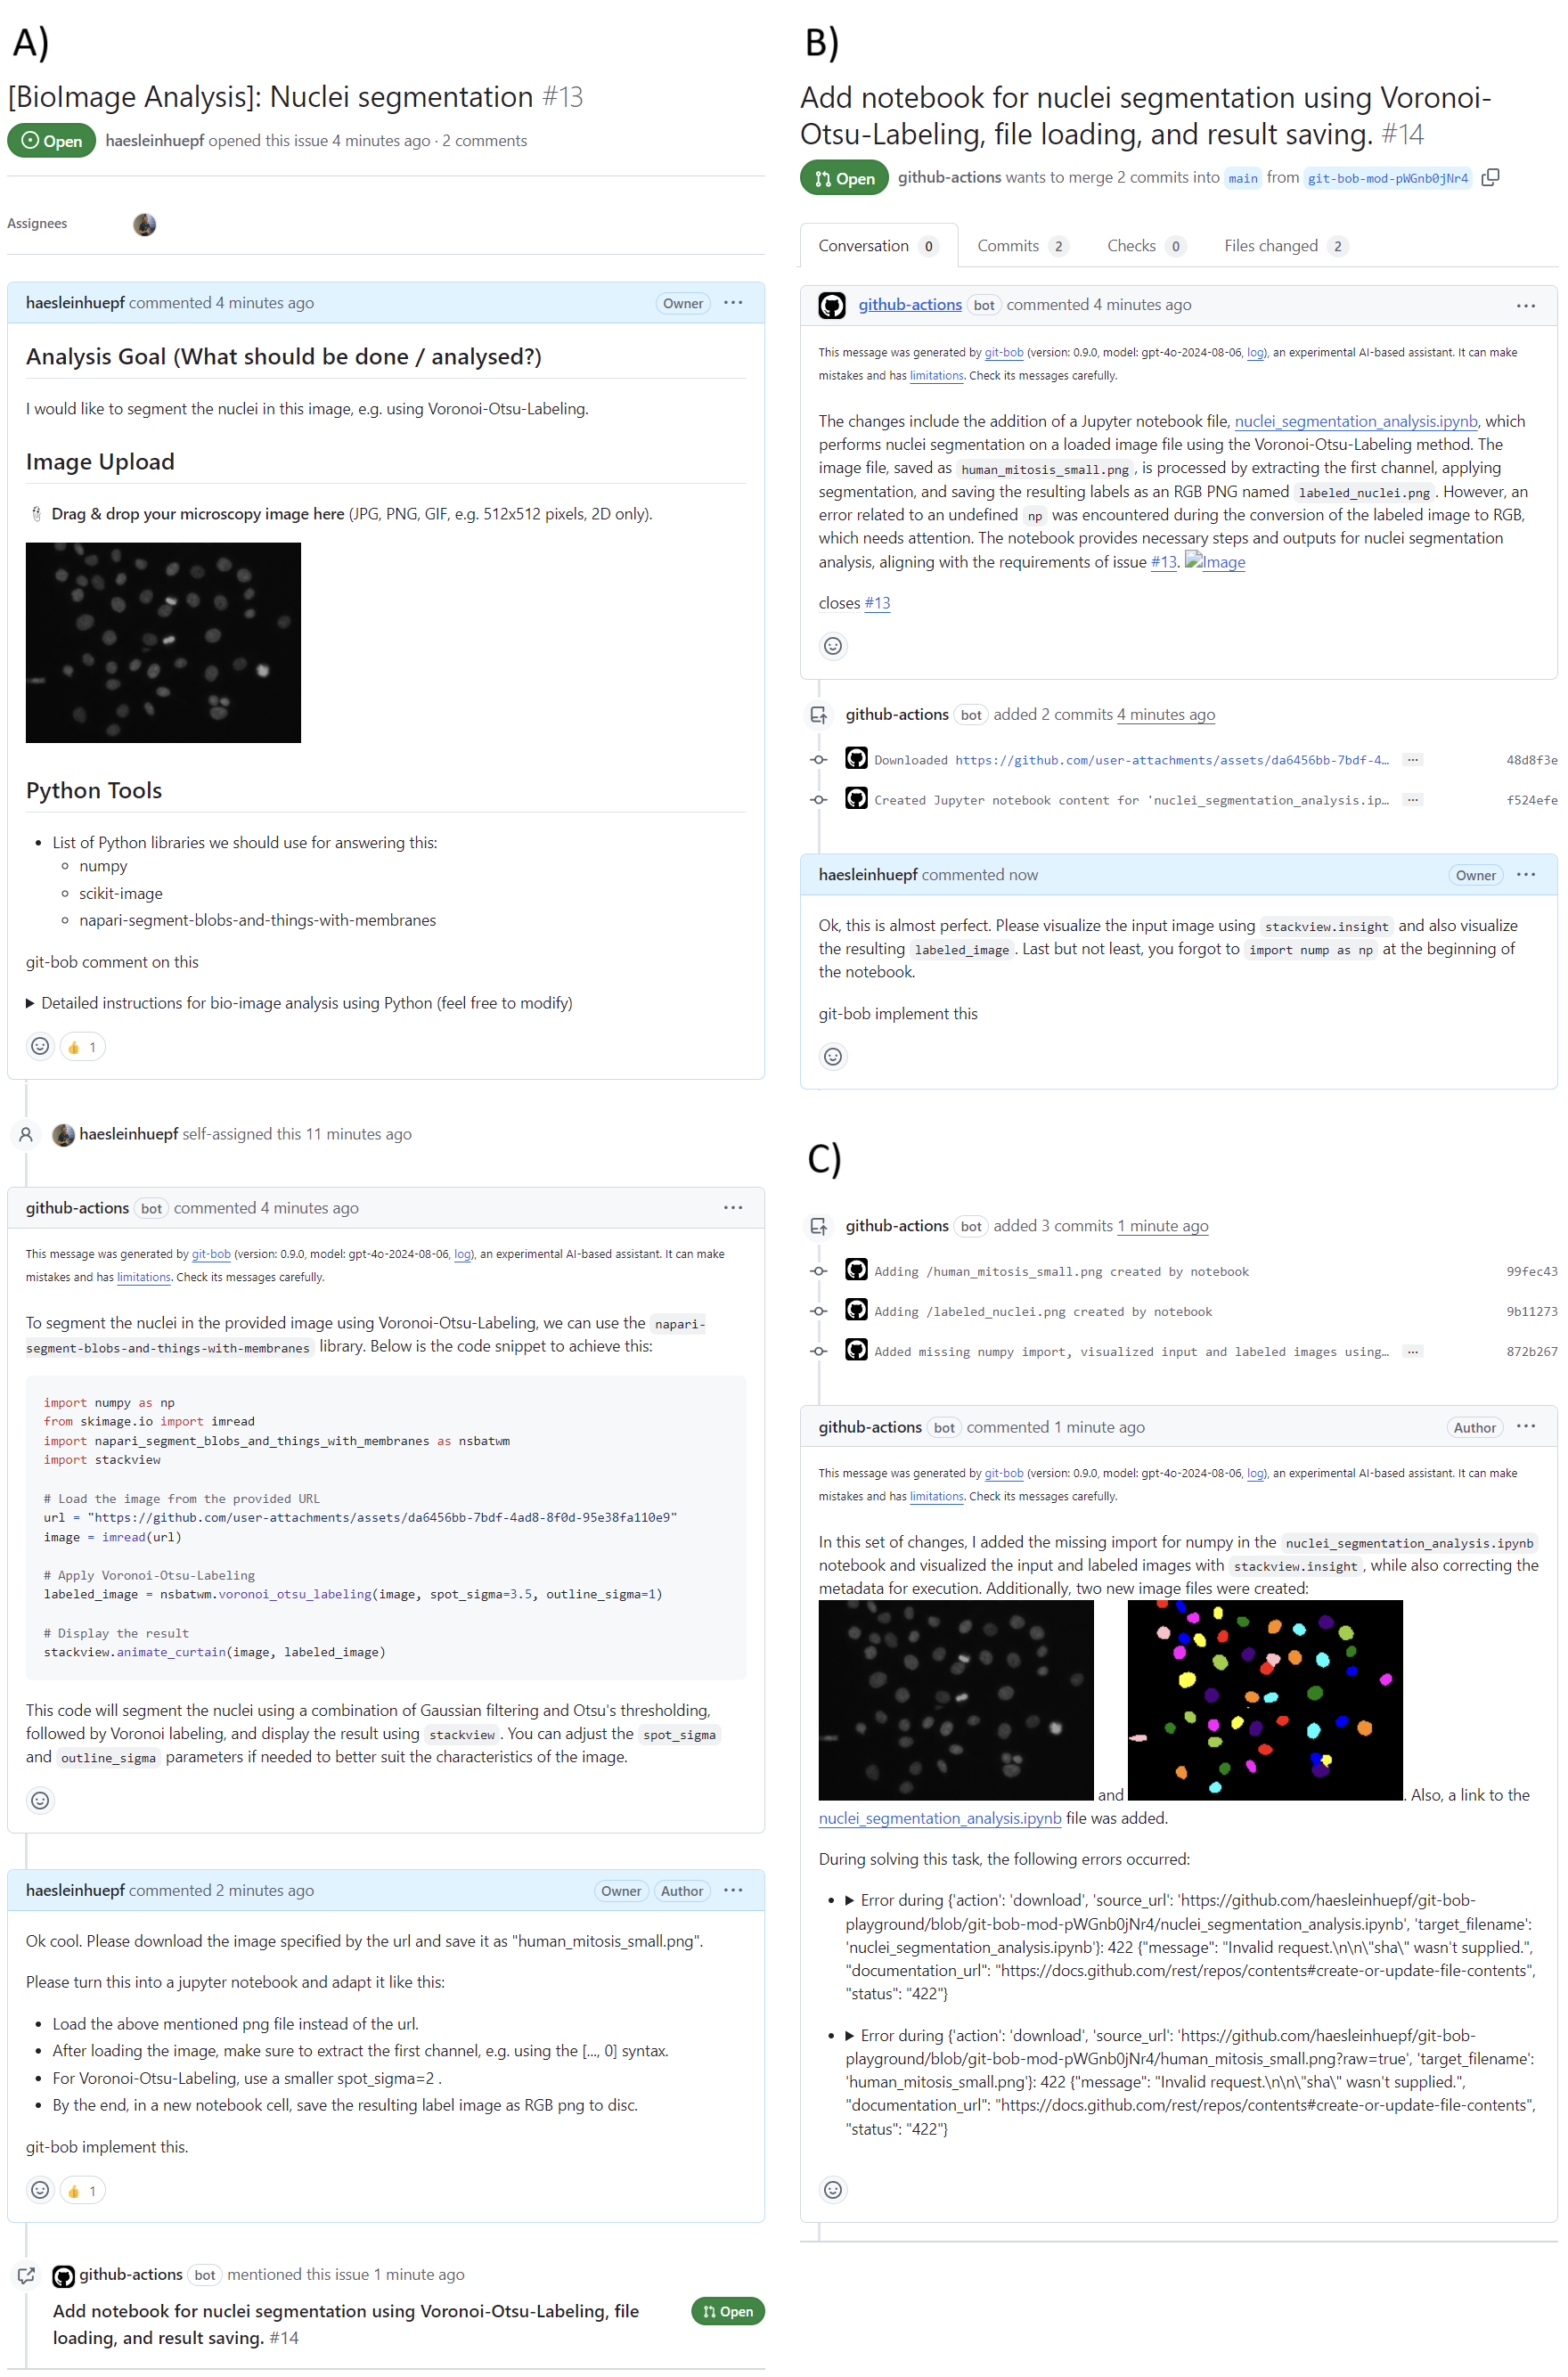
\includegraphics[width=0.5\textwidth]{example_interaction.png}
\caption{\textbf{Schematic view of the interaction with git-bob:} In one discussion thread, multiple humans (H) can interact with the AI-assistant, which is installed in GitHub or GitLab Continuous Integration (CI) infrastructure. Depending on how it is triggered, the AI-assistant may use LLMs from multiple LLM service providers in the background.
\newline
\newline
}
\label{fig:example_interaction}
\end{figure}

A schematic workflow involving git-bob is depicted in Figure \ref{fig:example_interaction}: a domain expert opens an issue, a type of discussion thread, on a repository on GitHub, where git-bob is installed. A repository member can then add more information to the request and trigger git-bob to answer by writing a command such as ``git-bob comment''. If externals try so, an automatic response will inform them that only repository members are allowed to trigger git-bob because running git-bob may cause costs for repository owners. Once triggered, git-bob will use an LLM to respond to the question, potentially including a code snippet and resulting plots or images. Users and the AI-assistant can then discuss back and forth until some potential solution is reached. This way, good-scientific-practice can be maintained by involving not just domain experts but also data analysis experts in the discussion. Optionally, git-bob can then be asked to implement the solution and send a GitHub pull-request, another type of discussion thread, but accompanied by file modifications to the repository, for instance, including a Jupyter Notebook containing the previously discussed code solution to a given issue. A human would need to review this pull-request and merge it into the code base of the repository. Git-bob also has the capability to review pull-requests originating from humans, but it is not allowed to merge them. This reflects established practices in science, where eventually a scientist is responsible for data analysis code that becomes part of the project. 

Common tasks git-bob is capable of are: \begin{itemize}
  \item Giving advice on how to solve a data analysis or data visualization task (\ref{fig:examplepairplot})
  \item Supporting users of open source libraries by providing advice and code examples, as shown in \ref{fig:examplesupportingusers}. As prompt engineering techniques have the potential to decrease wrong answers and halucinations \cite{yin2023largelanguagemodelsknow}, also git-bob can be instructed to forward the question to a human in case of doubt (\ref{fig:examplesupportingusers2}). It shall be noted that there is no garantee that the LLM makes this choice with perfect accuracy. 
  \item Documenting code (\ref{fig:example_add_documentation}). Such a task can be time-consuming when performed without AI-assistance, which can generate documentation for multiple Python functions in seconds to minutes. 
  \item Analysing data in the repository directly, and summarizing and plotting data in CSV files (\ref{fig:exampleplotting}). 
  \item Assisting in writing if manuscript files are stored in a GitHub repository, for example in latex format, git-bob can assist in writing. For example, the abstract for this manuscript was written by the AI-assistant and this is documented transparently as shown in \ref{fig:xample_abstract_generation}.
  \end{itemize}

A highlight of git-bob is that a local installation is not required. Git-bob is implemented as GitHub workflow or GitLab pipeline, which can be installed by uploading a configuration file to a repository and setting access rights. It is compatible and was tested with the commercial LLMs OpenAI's GPT4-omni, Anthropic's Claude 3.5 Sonnet, Google Gemini 1.5 Pro 002, and freely available models hosted on GitHub Models Marketplace. Git-bob reports which model was used in all of its messages, as good scientific practice suggests. Obviously, the communication with the selected LLM is transmitted to the service provider, including source code files from the repository and images provided with the GitHub issue. Hence, users are recommended to not submit any personal or sensitive information. When writing data analysis code, git-bob is intrinsically limited by the capabilities of the used LLM. For example, it has been shown that state-of-the-art (SOTA) LLMs can solve bio-image analysis questions by generating functionally correct code just above $50\%$ of tested cases \cite{benchmark_llm_bia}. This fundamental limitation may disappear when improved LLMs are published. For now, this can be evaded by the humans guiding the AI-assitant in multi-turn interactions towards a workable solution. Further technical limitations arise form prompt-length limitations of the underlying LLMs. When modifying or generating a file, these files must be below specified limits, for example GPT4-omni has $128k$ tokens input and $16k$ output tokens as limit (1 token $\approx$ approx. 3/4 words). Also when processing data, limitations of the GitHub IT infrastructure have to be considered: Git-bob executed in public repositories runs on virtual machines with 4 CPU cores, 16 GB of RAM and 14 GB of SSD storage. In private repositories, only 2 CPU cores and 7 GB RAM are available \cite{github_actions_runners_2024}. More capable systems are available on a paid basis. By installing git-bob in an institutional GitLab server, users can setup freely chosen hardware to run git-bob on.


\backmatter

\bmhead{Supplementary information}

Suppementary Figures are available in a separate document.

\bmhead{Acknowledgements}

I would like to thank Elena Katharina Nicolay (UFZ Leipzig) for testing git-bob in its early days and for providing constructive feedback on the manuscript. I also would like to thank Volker Hilsenstein for pushing for GitLab interoperability.

\section*{Declarations}

\begin{itemize}
\item Funding: I acknowledge the financial support by the Federal Ministry of Education and Research of Germany and by Sächsische Staatsministerium für Wissenschaft, Kultur und Tourismus in the programme Center of Excellence for AI-research "Center for Scalable Data Analytics and Artificial Intelligence Dresden/Leipzig", project identification number: ScaDS.AI. I also acknowledge financial support from the Deutsche Forschungsgemeinschaft (DFG, German Research Foundation) under the National Research Data Infrastructure – NFDI 46/1 – 501864659 - NFDI4BioImage.
\item Conflict of interest/Competing interests: The authors declare no conflict of interest.
\item Ethics approval and consent to participate: Not applicable.
\item Consent for publication: Consent.
\item Data availability: Not applicable.
\item Materials availability: Not applicable.
\item Code availability: The complete source code of git-bob is available online: https://github.com/haesleinhuepf/git-bob . The manuscipt is available openly too: https://github.com/haesleinhuepf/git-bob-manuscript
\item Author contribution: RH wrote the software and the manuscript. Some portions of code and text were generated using generative artificial intelligence. The git-history of the both above mentioned repositories informs about which parts were written by RH: Parts which parts were AI-generated are authored by github-actions[bot].
\end{itemize}

\noindent

%%===================================================%%
%% For presentation purpose, we have included        %%
%% \bigskip command. Please ignore this.             %%
%%===================================================%%
\bigskip


\begin{appendices}


%%%%%%%%%%%%%%%%%%%%%%%%%%%%%
% Supplementary Information %
%%%%%%%%%%%%%%%%%%%%%%%%%%%%%
%\captionsetup*{format=largeformat}


\onecolumn
\newpage

\section*{Supplementary Information}
\setcounter{figure}{0} 
\renewcommand{\figurename}{}
\renewcommand{\thefigure}{Supplementary Figure \arabic{figure}}


\begin{figure*}[h]
\centering
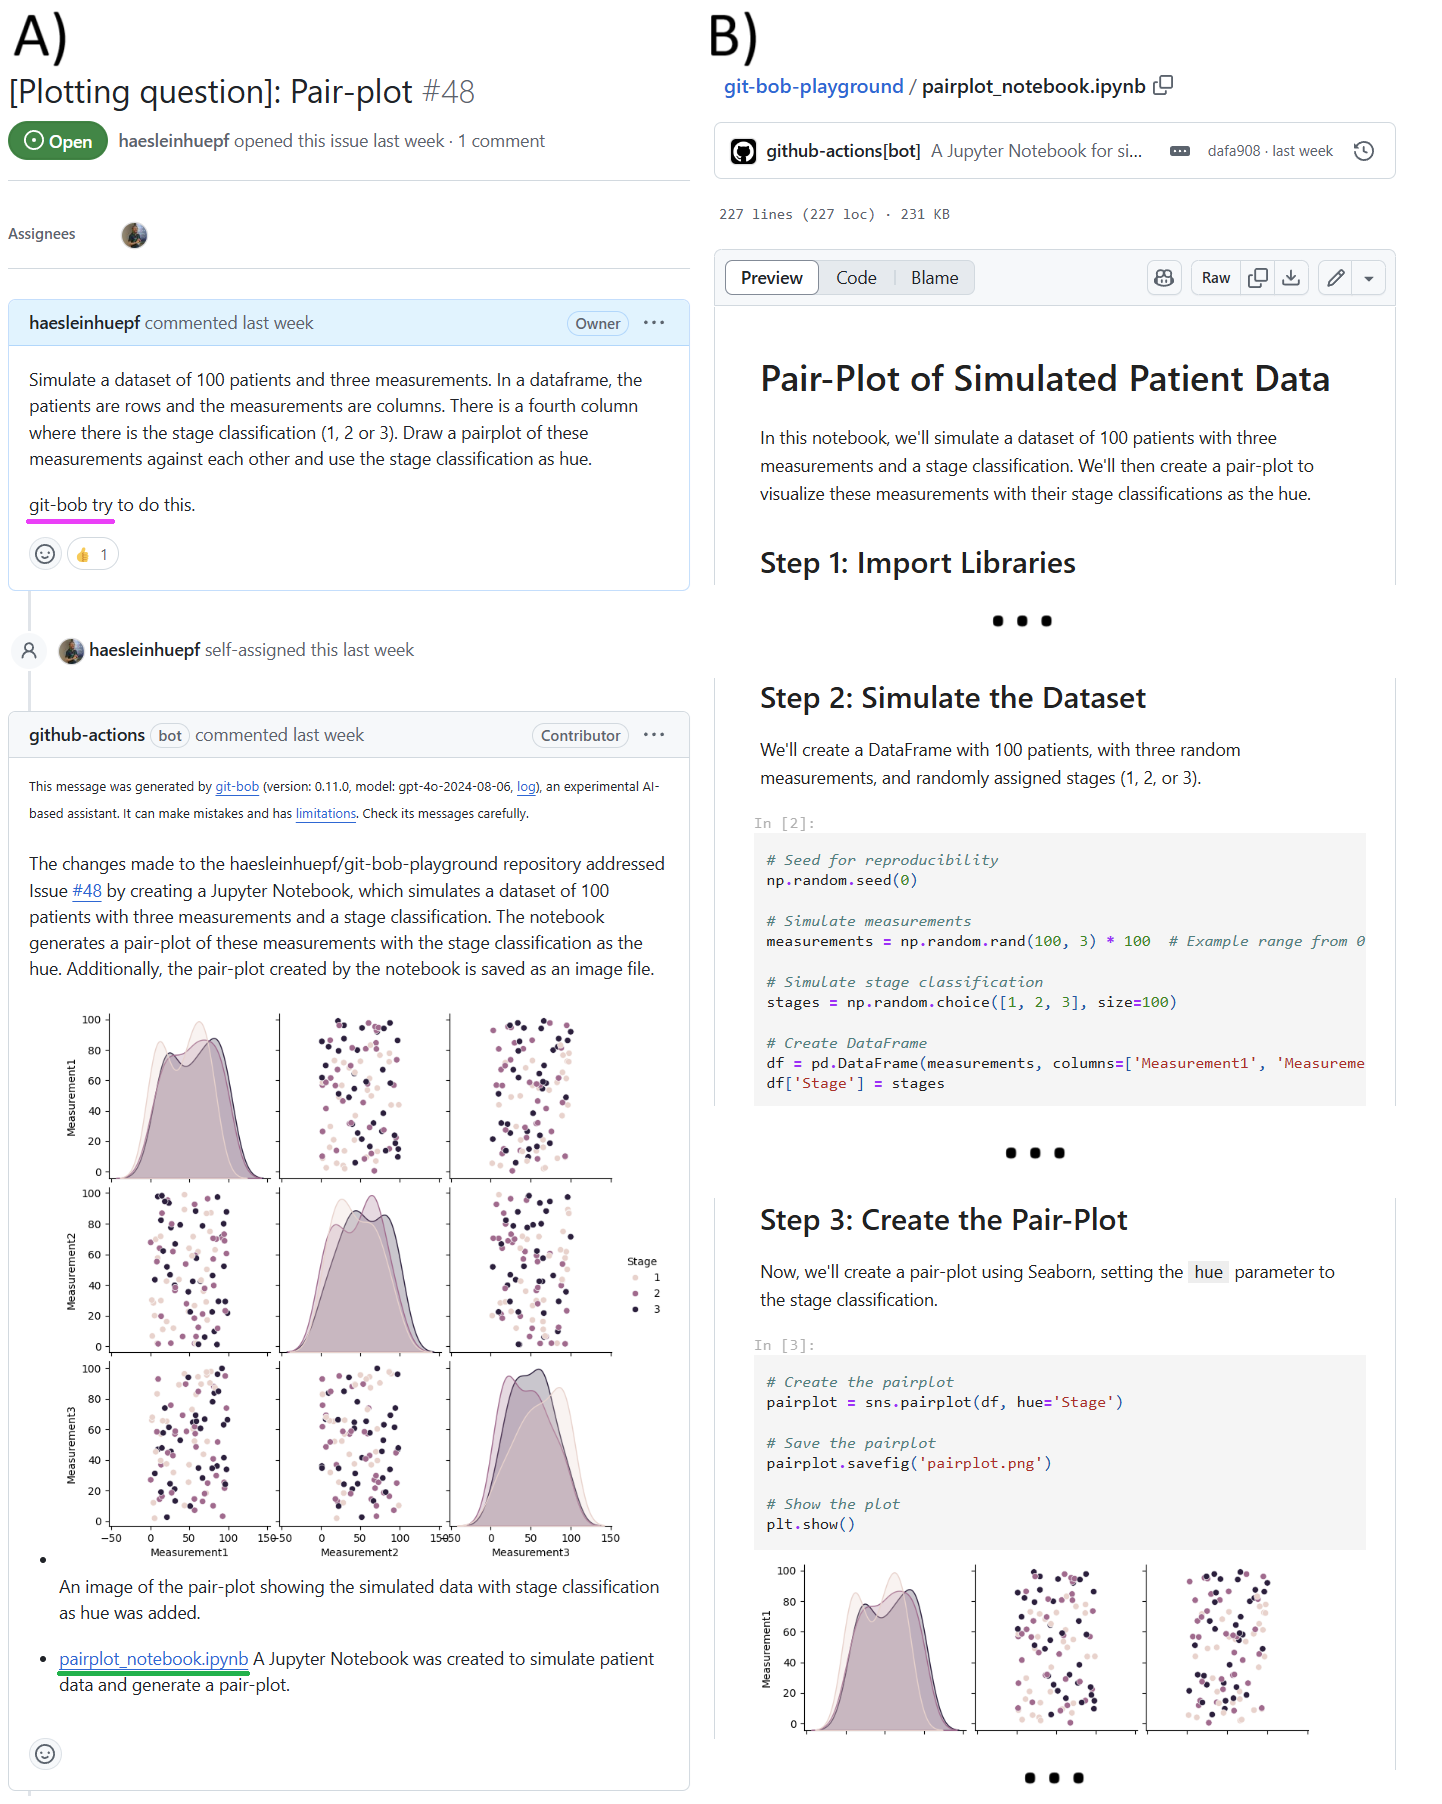
\includegraphics[width=0.9\textwidth]{example_pair_plot.png}
\caption{\textbf{Use-case example for generating data analysis code:} The user explains a scenario (A) and triggers git-bob (underlined in magenta). The AI-assistant generates and executes code and visualizes the resulting plot. The user can click on the link to the generated notebook (underlined in green) to go to the notebook (B) and read the code and see intermediate results. The shown notebook is an excerpt as indicated by ``...''. The entire discussion and corresponding code can be read online: \url{https://github.com/haesleinhuepf/git-bob-playground/issues/48}
\newline
\newline
}
\label{fig:examplepairplot}
\end{figure*}


\begin{figure*}[h]
\centering
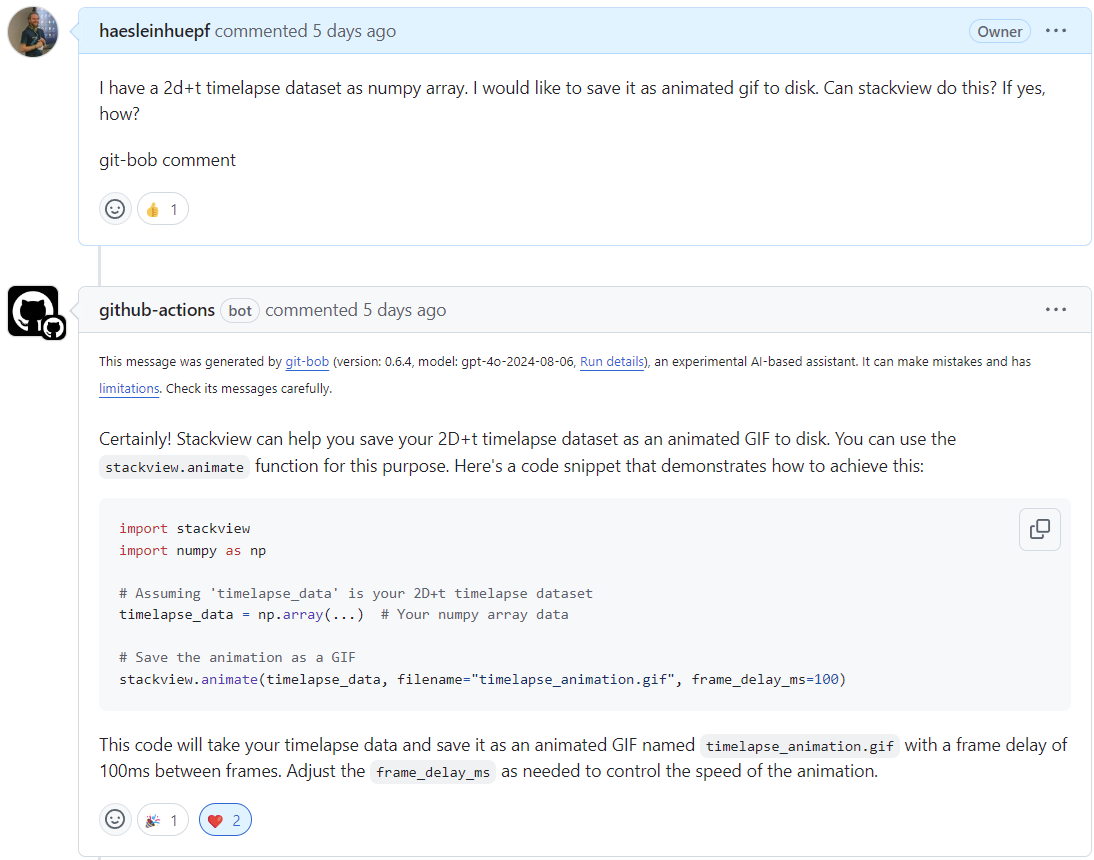
\includegraphics[width=0.8\textwidth]{example_supporting_users.png}
\caption{\textbf{Use-case example for supporting users:} The assistant can be configured to act as expert on a specific Python library and answer user questions. Words triggering git-bob are underlined in magenta. The entire discussion and corresponding code can be read online: \url{https://github.com/haesleinhuepf/stackview/issues/79}
\newline
\newline
}
\label{fig:examplesupportingusers}
\end{figure*}


\begin{figure*}[h]
\centering
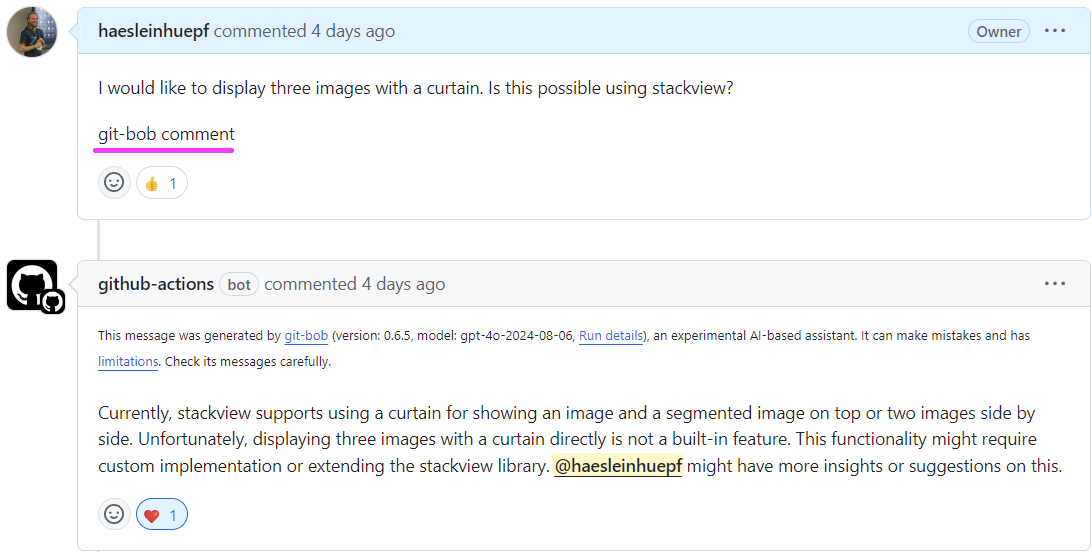
\includegraphics[width=0.8\textwidth]{example_supporting_users2.png}
\caption{\textbf{Use-case example for asking an expert:} The answer to the question shown here is "No", but this is nowhere written in the documentation or the configuration of the assistant. In this case the assistant is not sure, and it can be configured to forward a question to a maintainer of the library where the question arrived. Words triggering git-bob are underlined in magenta. The entire discussion and corresponding code can be read online: \url{https://github.com/haesleinhuepf/stackview/issues/80}
\newline
\newline
}
\label{fig:examplesupportingusers2}
\end{figure*}



\begin{figure*}[h]
\centering
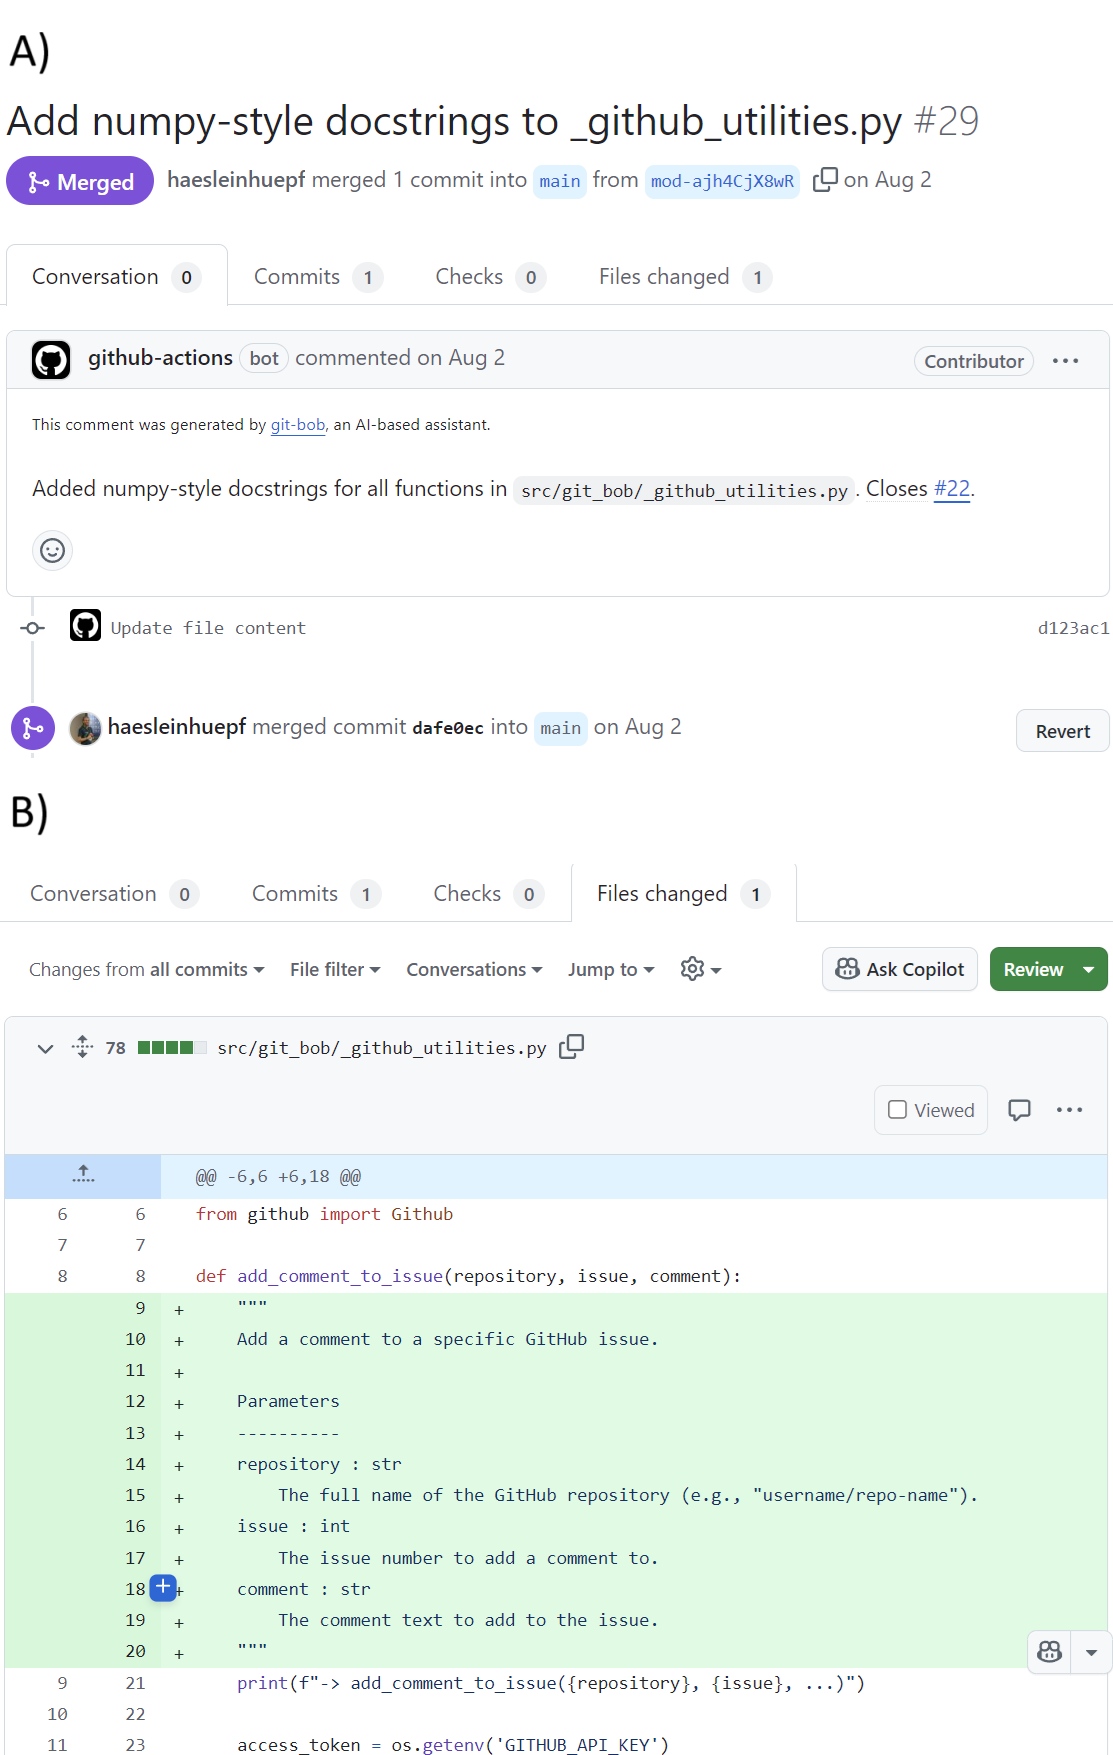
\includegraphics[width=0.82\textwidth]{example_add_documentation.png}
\caption{\textbf{Use-case example for adding and revising documentation in code:} git-bob was used to partially write the code documentation of its own code. When asked to add documentation in a specific format, it sent a pull-request (A) and the human could inspect the code modifications (B, excerpt) before mergin the code into the project's code base. The entire discussion and corresponding code can be read online: \url{https://github.com/haesleinhuepf/git-bob/pull/29}
\newline
\newline
}
\label{fig:example_add_documentation}
\end{figure*}


\begin{figure*}[h]
\centering
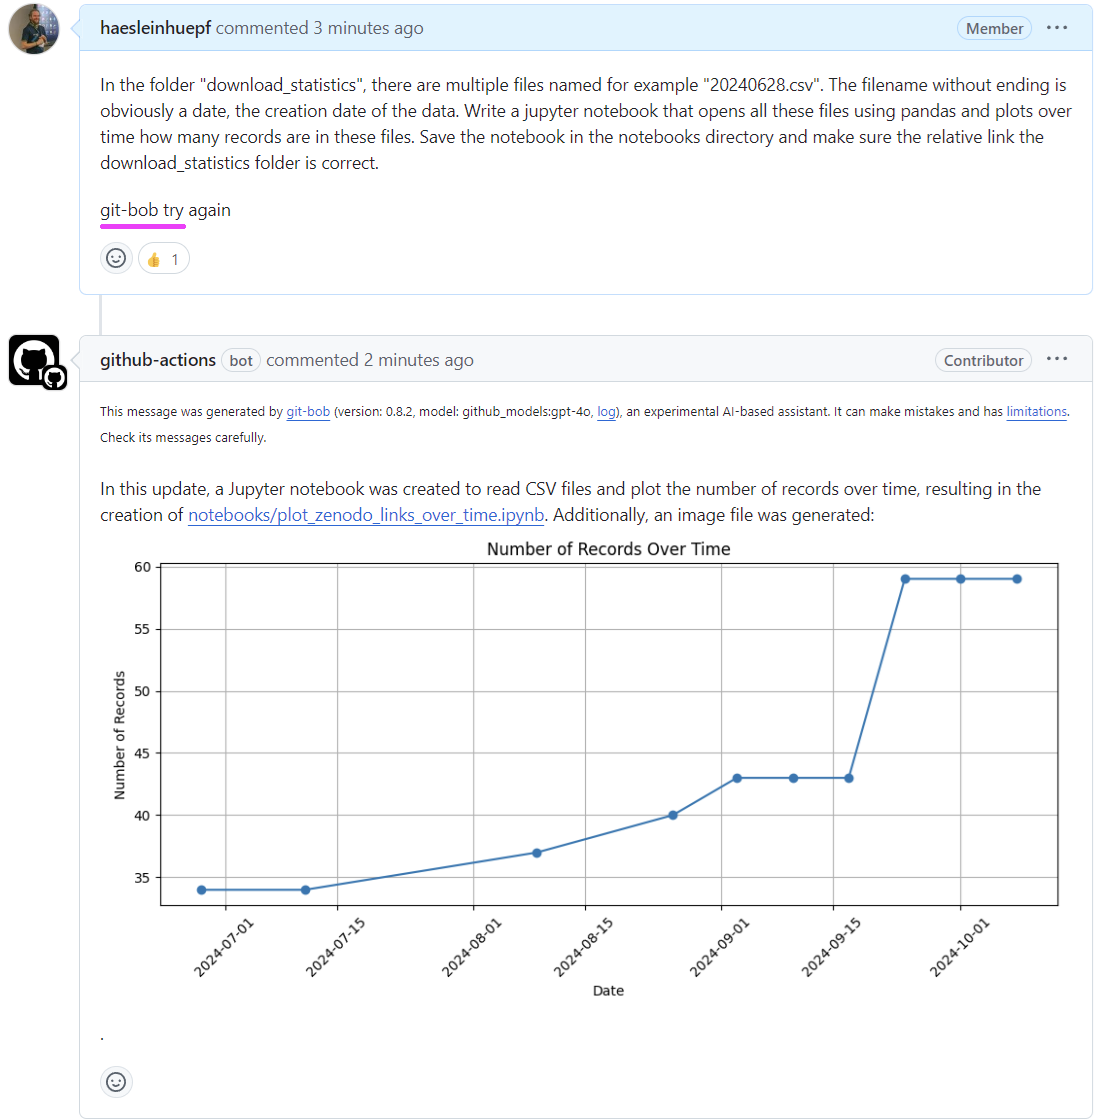
\includegraphics[width=\textwidth]{example_plotting.png}
\caption{\textbf{Use-case example for plotting data:} after explaining the assistant the folder structure of the project, it generates code for parsing a folder of CSV files and plotting results. Words triggering git-bob are underlined in magenta. The entire discussion and corresponding code can be read online: \url{https://github.com/NFDI4BIOIMAGE/training/issues/250}
\newline
\newline
}
\label{fig:exampleplotting}
\end{figure*}






\begin{figure*}[h]
\centering
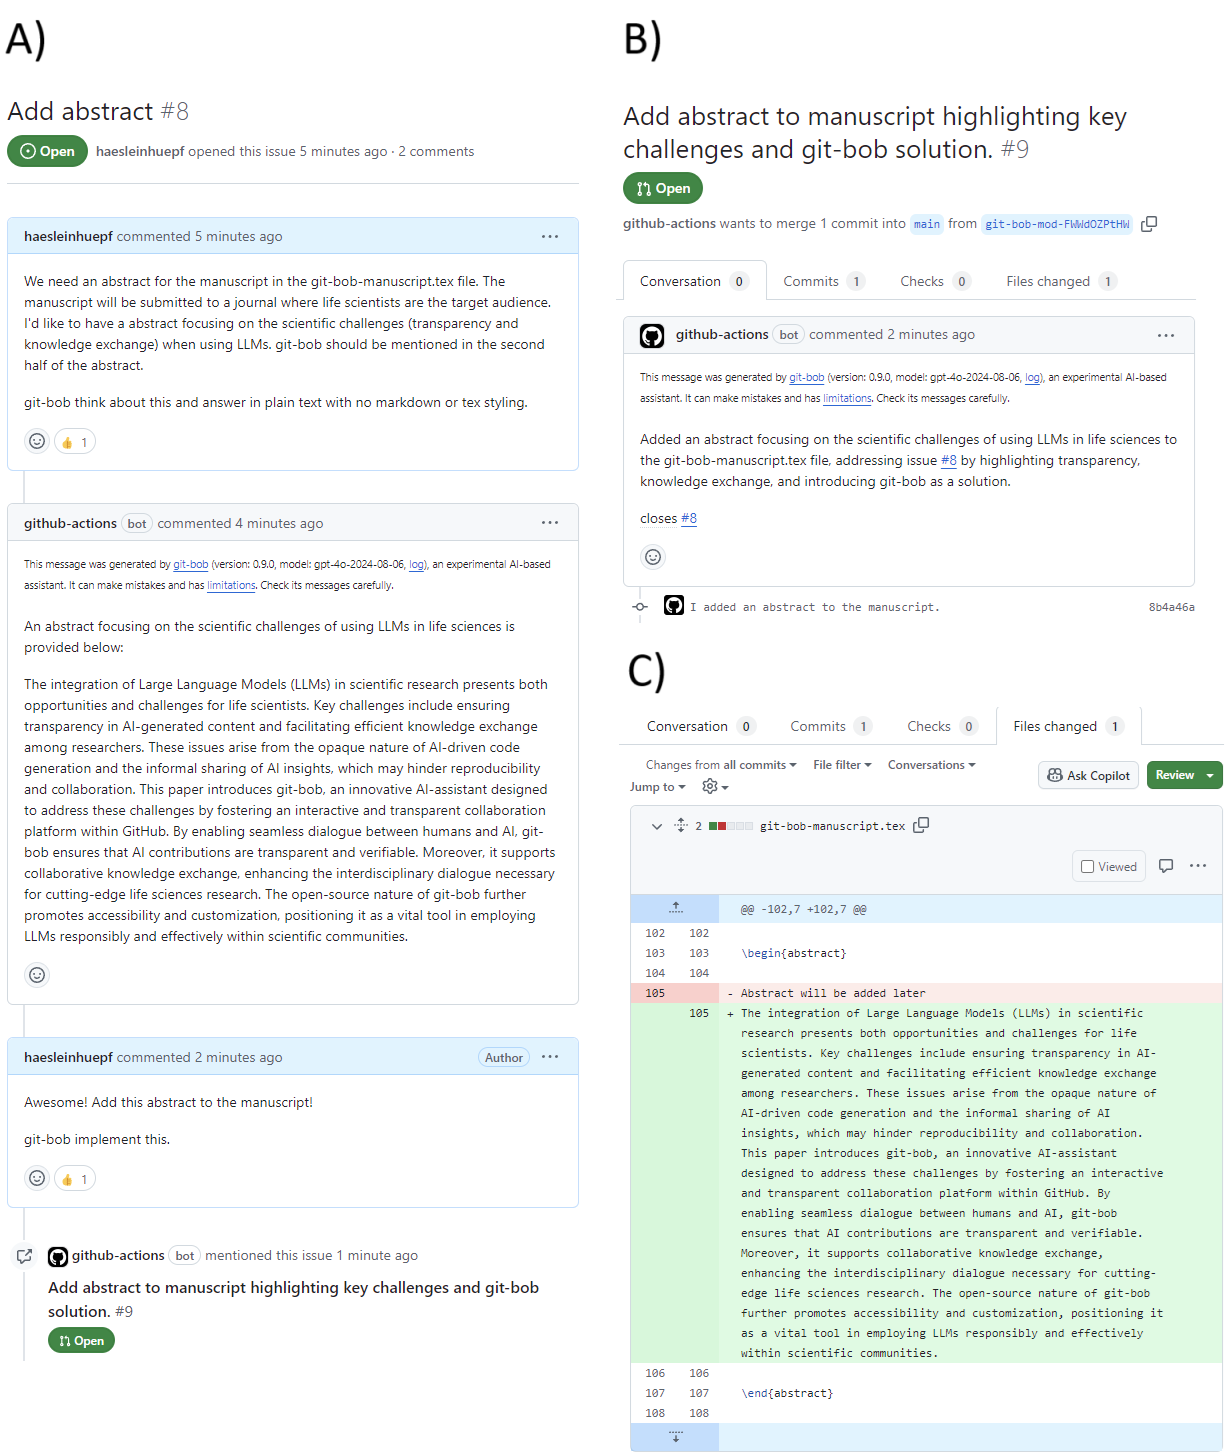
\includegraphics[width=\textwidth]{example_abstract_generation.png}
\caption{\textbf{Use-case example for working on scientific manuscripts:} after a first draft of the manuscript was written, git-bob was asked to formulate an abstract (A). The abstract was then submitted as pull-request with a short description (B). The human can also review and potentially modify the proposed text in this online interface (C). Words triggering git-bob are underlined in magenta. The entire discussion can be read online: \url{https://github.com/haesleinhuepf/git-bob-manuscript/issues/8} and \url{https://github.com/haesleinhuepf/git-bob-manuscript/pull/9}.
\newline
\newline
}
\label{fig:xample_abstract_generation}
\end{figure*}

\end{appendices}

%%===========================================================================================%%
%% If you are submitting to one of the Nature Portfolio journals, using the eJP submission   %%
%% system, please include the references within the manuscript file itself. You may do this  %%
%% by copying the reference list from your .bbl file, paste it into the main manuscript .tex %%
%% file, and delete the associated \verb+\bibliography+ commands.                            %%
%%===========================================================================================%%

%%\bibliography{mybibfile}% common bib file
%% if required, the content of .bbl file can be included here once bbl is generated
%%\input sn-article.bbl

%% BioMed_Central_Bib_Style_v1.01

\begin{thebibliography}{10}
% BibTex style file: bmc-mathphys.bst (version 2.1), 2014-07-24
\ifx \bisbn   \undefined \def \bisbn  #1{ISBN #1}\fi
\ifx \binits  \undefined \def \binits#1{#1}\fi
\ifx \bauthor  \undefined \def \bauthor#1{#1}\fi
\ifx \batitle  \undefined \def \batitle#1{#1}\fi
\ifx \bjtitle  \undefined \def \bjtitle#1{#1}\fi
\ifx \bvolume  \undefined \def \bvolume#1{\textbf{#1}}\fi
\ifx \byear  \undefined \def \byear#1{#1}\fi
\ifx \bissue  \undefined \def \bissue#1{#1}\fi
\ifx \bfpage  \undefined \def \bfpage#1{#1}\fi
\ifx \blpage  \undefined \def \blpage #1{#1}\fi
\ifx \burl  \undefined \def \burl#1{\textsf{#1}}\fi
\ifx \doiurl  \undefined \def \doiurl#1{\url{https://doi.org/#1}}\fi
\ifx \betal  \undefined \def \betal{\textit{et al.}}\fi
\ifx \binstitute  \undefined \def \binstitute#1{#1}\fi
\ifx \binstitutionaled  \undefined \def \binstitutionaled#1{#1}\fi
\ifx \bctitle  \undefined \def \bctitle#1{#1}\fi
\ifx \beditor  \undefined \def \beditor#1{#1}\fi
\ifx \bpublisher  \undefined \def \bpublisher#1{#1}\fi
\ifx \bbtitle  \undefined \def \bbtitle#1{#1}\fi
\ifx \bedition  \undefined \def \bedition#1{#1}\fi
\ifx \bseriesno  \undefined \def \bseriesno#1{#1}\fi
\ifx \blocation  \undefined \def \blocation#1{#1}\fi
\ifx \bsertitle  \undefined \def \bsertitle#1{#1}\fi
\ifx \bsnm \undefined \def \bsnm#1{#1}\fi
\ifx \bsuffix \undefined \def \bsuffix#1{#1}\fi
\ifx \bparticle \undefined \def \bparticle#1{#1}\fi
\ifx \barticle \undefined \def \barticle#1{#1}\fi
\bibcommenthead
\ifx \bconfdate \undefined \def \bconfdate #1{#1}\fi
\ifx \botherref \undefined \def \botherref #1{#1}\fi
\ifx \url \undefined \def \url#1{\textsf{#1}}\fi
\ifx \bchapter \undefined \def \bchapter#1{#1}\fi
\ifx \bbook \undefined \def \bbook#1{#1}\fi
\ifx \bcomment \undefined \def \bcomment#1{#1}\fi
\ifx \oauthor \undefined \def \oauthor#1{#1}\fi
\ifx \citeauthoryear \undefined \def \citeauthoryear#1{#1}\fi
\ifx \endbibitem  \undefined \def \endbibitem {}\fi
\ifx \bconflocation  \undefined \def \bconflocation#1{#1}\fi
\ifx \arxivurl  \undefined \def \arxivurl#1{\textsf{#1}}\fi
\csname PreBibitemsHook\endcsname

%%% 1
\bibitem[\protect\citeauthoryear{Royer}{2023}]{Royer2023}
\begin{barticle}
\bauthor{\bsnm{Royer}, \binits{L.A.}}:
\batitle{The future of bioimage analysis: a dialog between mind and machine}.
\bjtitle{Nature Methods}
\bvolume{20}(\bissue{7}),
\bfpage{951}--\blpage{952}
(\byear{2023})
\doiurl{10.1038/s41592-023-01930-y}
\end{barticle}
\endbibitem

%%% 2
\bibitem[\protect\citeauthoryear{Lai et~al.}{2022}]{Lai2022DS1000}
\begin{botherref}
\oauthor{\bsnm{Lai}, \binits{Y.}},
\oauthor{\bsnm{Li}, \binits{C.}},
\oauthor{\bsnm{Wang}, \binits{Y.}},
\oauthor{\bsnm{Zhang}, \binits{T.}},
\oauthor{\bsnm{Zhong}, \binits{R.}},
\oauthor{\bsnm{Zettlemoyer}, \binits{L.}},
\oauthor{\bsnm{Yih}, \binits{S.W.-t.}},
\oauthor{\bsnm{Fried}, \binits{D.}},
\oauthor{\bsnm{Wang}, \binits{S.}},
\oauthor{\bsnm{Yu}, \binits{T.}}:
DS-1000: A Natural and Reliable Benchmark for Data Science Code Generation
(2022)
\end{botherref}
\endbibitem

%%% 3
\bibitem[\protect\citeauthoryear{Lei et~al.}{2024}]{lei2024bioimage}
\begin{barticle}
\bauthor{\bsnm{Lei}, \binits{W.}},
\bauthor{\bsnm{Fuster-Barcel{\'o}}, \binits{C.}},
\bauthor{\bsnm{Reder}, \binits{G.}}, \betal:
\batitle{Bioimage.io chatbot: a community-driven ai assistant for integrative
  computational bioimaging}.
\bjtitle{Nature Methods}
\bvolume{21},
\bfpage{1368}--\blpage{1370}
(\byear{2024})
\doiurl{10.1038/s41592-024-02370-y}
\end{barticle}
\endbibitem

%%% 4
\bibitem[\protect\citeauthoryear{Royer}{2024}]{Royer2024}
\begin{barticle}
\bauthor{\bsnm{Royer}, \binits{L.A.}}:
\batitle{Omega — harnessing the power of large language models for bioimage
  analysis}.
\bjtitle{Nature Methods}
\bvolume{21}(\bissue{8}),
\bfpage{1371}--\blpage{1373}
(\byear{2024})
\doiurl{10.1038/s41592-024-02310-w}
\end{barticle}
\endbibitem

%%% 5
\bibitem[\protect\citeauthoryear{Haase et~al.}{2024}]{benchmark_llm_bia}
\begin{barticle}
\bauthor{\bsnm{Haase}, \binits{R.}},
\bauthor{\bsnm{Tischer}, \binits{C.}},
\bauthor{\bsnm{H{\'e}rich{\'e}}, \binits{J.-K.}},
\bauthor{\bsnm{Scherf}, \binits{N.}}:
\batitle{Benchmarking large language models for bio-image analysis code
  generation}.
\bjtitle{bioRxiv}
(\byear{2024})
\doiurl{10.1101/2024.04.19.590278}
{\href{https://arxiv.org/abs/https://www.biorxiv.org/content/early/2024/04/25/2024.04.19.590278.full.pdf}{{https://www.biorxiv.org/content/early/2024/04/25/2024.04.19.590278.full.pdf}}}
\end{barticle}
\endbibitem

%%% 6
\bibitem[\protect\citeauthoryear{Chen et~al.}{2021}]{chen2021evaluating}
\begin{botherref}
\oauthor{\bsnm{Chen}, \binits{M.}},
\oauthor{\bsnm{Tworek}, \binits{J.}},
\oauthor{\bsnm{Jun}, \binits{H.}},
\oauthor{\bsnm{Yuan}, \binits{Q.}},
\oauthor{\bsnm{Oliveira~Pinto}, \binits{H.P.}}, et al.:
Evaluating large language models trained on code.
CoRR
\textbf{abs/2107.03374}
(2021)
{\href{https://arxiv.org/abs/2107.03374}{{2107.03374}}}
\end{botherref}
\endbibitem

%%% 7
\bibitem[\protect\citeauthoryear{Lu et~al.}{2024}]{lu2024aiscientist}
\begin{botherref}
\oauthor{\bsnm{Lu}, \binits{C.}},
\oauthor{\bsnm{Lu}, \binits{C.}},
\oauthor{\bsnm{Lange}, \binits{R.T.}},
\oauthor{\bsnm{Foerster}, \binits{J.}},
\oauthor{\bsnm{Clune}, \binits{J.}},
\oauthor{\bsnm{Ha}, \binits{D.}}:
The {AI} {S}cientist: Towards fully automated open-ended scientific discovery.
arXiv preprint arXiv:2408.06292
(2024)
\end{botherref}
\endbibitem

%%% 8
\bibitem[\protect\citeauthoryear{Jimenez
  et~al.}{2024}]{jimenez2024swebenchlanguagemodelsresolve}
\begin{botherref}
\oauthor{\bsnm{Jimenez}, \binits{C.E.}},
\oauthor{\bsnm{Yang}, \binits{J.}},
\oauthor{\bsnm{Wettig}, \binits{A.}},
\oauthor{\bsnm{Yao}, \binits{S.}},
\oauthor{\bsnm{Pei}, \binits{K.}},
\oauthor{\bsnm{Press}, \binits{O.}},
\oauthor{\bsnm{Narasimhan}, \binits{K.}}:
SWE-bench: Can Language Models Resolve Real-World GitHub Issues?
(2024).
\url{https://arxiv.org/abs/2310.06770}
\end{botherref}
\endbibitem

%%% 9
\bibitem[\protect\citeauthoryear{Yin
  et~al.}{2023}]{yin2023largelanguagemodelsknow}
\begin{botherref}
\oauthor{\bsnm{Yin}, \binits{Z.}},
\oauthor{\bsnm{Sun}, \binits{Q.}},
\oauthor{\bsnm{Guo}, \binits{Q.}},
\oauthor{\bsnm{Wu}, \binits{J.}},
\oauthor{\bsnm{Qiu}, \binits{X.}},
\oauthor{\bsnm{Huang}, \binits{X.}}:
Do Large Language Models Know What They Don't Know?
(2023).
\url{https://arxiv.org/abs/2305.18153}
\end{botherref}
\endbibitem

%%% 10
\bibitem[\protect\citeauthoryear{GitHub}{2024}]{github_actions_runners_2024}
\begin{botherref}
\oauthor{\bsnm{GitHub}}:
About GitHub-hosted Runners
  \url{https://docs.github.com/en/actions/using-github-hosted-runners/using-github-hosted-runners/about-github-hosted-runners}.
Accessed: 2024-10-14
(2024).
\url{https://docs.github.com/en/actions/using-github-hosted-runners/using-github-hosted-runners/about-github-hosted-runners}
\end{botherref}
\endbibitem

\end{thebibliography}


\end{document}

